% ------------------------------------------------------------------------------
% TYPO3 Version 10.3 - What's New (German Version)
%
% @license	Creative Commons BY-NC-SA 3.0
% @link		https://typo3.org/help/documentation/whats-new/
% @language	German
% ------------------------------------------------------------------------------

\section{Änderungen für Entwickler}
\begin{frame}[fragile]
	\frametitle{Änderungen für Entwickler}

	\begin{center}\huge{Kapitel 3:}\end{center}
	\begin{center}\huge{\color{typo3darkgrey}\textbf{Änderungen für Entwickler}}\end{center}

\end{frame}

% ------------------------------------------------------------------------------
% Feature | 90333 | Dashboard

\begin{frame}[fragile]
	\frametitle{Änderungen für Entwickler}
	\framesubtitle{Dashboard (1)}

	% decrease font size for code listing
	\lstset{basicstyle=\smaller\ttfamily}

	\begin{itemize}
		\item Entwickler können benutzdefinierte Widgets für das Dashboard erstellen, indem sie eine der folgenden  Widget \textit{abstracts} erweitern:

			\begin{itemize}
				\item \texttt{AbstractWidget}\newline
					\small
						Kann als Anfang von einfachen Widgets verwendet werden.
					\normalsize
				\item \texttt{AbstractRssWidget}\newline
					\small
						Wird zur Erstellung eines Widgets, das einen RSS-Feed anzeigt, benutzt.
					\normalsize
				\item \texttt{AbstractListWidget}\newline
					\small
						Ein Abstract zum Erstellen eines Widgets, das eine Liste von Elementen anzeigt.
					\normalsize
				\item \texttt{AbstractCtaButtonWidget}\newline
					\small
						Ein Abstract zum Erstellen eines Widgets, das ein "call-to-action" Button anzeigt.
					\normalsize
			\end{itemize}

	\end{itemize}

\end{frame}

% ------------------------------------------------------------------------------
% Feature | 90333 | Dashboard

\begin{frame}[fragile]
	\frametitle{Changes for Developers}
	\framesubtitle{Dashboard (2)}

	% decrease font size for code listing
	\lstset{basicstyle=\tiny\ttfamily}

	\begin{itemize}
		\item Registrieren Sie Ihre Widgets in der folgenden Zeile Ihrer Erweiterung:\newline
			\texttt{EXT:my\_extension/Configuration/Services.yaml}

		\item Option 1: Widgetbezeichner als Attribut

\vspace{-0.4cm}
\begin{lstlisting}
Vendor\MyExtension\Widgets\MyFirstWidget:
  tags:
    - name: dashboard.widget
      identifier: widget-identifier-1
      widgetGroups: 'general'
\end{lstlisting}

		\item Option 2: Der benutzerdefinierte Service-Name erlaubt es mehreren Widget-Identifikatoren, eine Klasse gemeinsam zu nutzen

\vspace{-0.4cm}
\begin{lstlisting}
widget.identifier:
  class: Vendor\MyExtension\Widgets\MySecondWidget
  tags:
    - name: dashboard.widget
      identifier: widget-identifier-2
      widgetGroups: 'general, typo3'
\end{lstlisting}

	\end{itemize}

\end{frame}

% ------------------------------------------------------------------------------
% Feature | 90333 | Dashboard

\begin{frame}[fragile]
	\frametitle{Änderungen für Entwickler}
	\framesubtitle{Dashboard (3)}

	% decrease font size for code listing
	\lstset{basicstyle=\tiny\ttfamily}

	\begin{itemize}
		\item Jedes Widget ist einer oder mehreren Widget-Gruppen zugeordnet.
		\item Diese Gruppen werden im Modal angezeigt, wenn Sie ein neues Widget zum Dashboard hinzufügen.
		\item Entwickler können benutzerdefinierte Widget-Gruppen konfigurieren, indem sie eine Datei erstellen\newline
			\smaller
				\texttt{EXT:my\_extension/Configuration/Backend/DashboardWidgetGroups.php}
			\normalsize

\vspace{-0.4cm}
\begin{lstlisting}
return [
  'widgetGroup-exampleGroup' => [
    'title' => 'LLL:EXT:my_extension/Resources/Private/Language/locallang.xlf:widget_group_name',
  ],
];
\end{lstlisting}

	\end{itemize}

\end{frame}

% ------------------------------------------------------------------------------
% Feature | 89870 | New PSR-14 Events for Extbase-related signals

\begin{frame}[fragile]
	\frametitle{Änderungen für Entwickler}
	\framesubtitle{Extbase und Fluid}

	% decrease font size for code listing
	\lstset{basicstyle=\tiny\ttfamily}

	\begin{itemize}
		\item Die folgenden PSR-14-basierten Events wurden für Extbase-bezogene Signale eingeführt:

\vspace{-0.4cm}
\begin{lstlisting}
TYPO3\CMS\Extbase\Event\Mvc\AfterRequestDispatchedEvent
TYPO3\CMS\Extbase\Event\Mvc\BeforeActionCallEvent
TYPO3\CMS\Extbase\Event\Persistence\AfterObjectThawedEvent
TYPO3\CMS\Extbase\Event\Persistence\ModifyQueryBeforeFetchingObjectDataEvent
TYPO3\CMS\Extbase\Event\Persistence\ModifyResultAfterFetchingObjectDataEvent
TYPO3\CMS\Extbase\Event\Persistence\EntityAddedToPersistenceEvent
TYPO3\CMS\Extbase\Event\Persistence\EntityFinalizedAfterPersistenceEvent
TYPO3\CMS\Extbase\Event\Persistence\EntityUpdatedInPersistenceEvent
TYPO3\CMS\Extbase\Event\Persistence\EntityRemovedFromPersistenceEvent
TYPO3\CMS\Extbase\Event\Persistence\EntityPersistedEvent
\end{lstlisting}

		\item Bestehende Signale wurden ersetzt und sollten nicht mehr verwendet werden.

	\end{itemize}

\end{frame}

% ------------------------------------------------------------------------------
% Feature | 89644 | Add optional argument fields to editRecord ViewHelpers

\begin{frame}[fragile]
	\frametitle{Änderungen für Entwickler}
	\framesubtitle{ViewHelper \texttt{editRecord}}

	% decrease font size for code listing
	\lstset{basicstyle=\tiny\ttfamily}

	\begin{itemize}
		\item Ein optionales Argument \texttt{fields} wurde den
			\texttt{uri.editRecord} und \texttt{link.editRecord} ViewHelpern hinzugefügt.
		\item Falls gesetzt, erstellt die FormEngine ein Formular, um nur das/die gegebene(n) Datenbankfeld(er) zu bearbeiten.
		\item Das folgende Beispiel erstellt einen Link, um das \texttt{tt\_content.bodytext}
			-Feld des Datensatzes mit der UID 42 zu bearbeiten.

\begin{lstlisting}
<be:link.editRecord uid="42" table="tt_content" fields="bodytext" returnUrl="foo/bar">
  Edit record
</be:link.editRecord>
\end{lstlisting}

	\end{itemize}

\end{frame}

% ------------------------------------------------------------------------------
% Feature | xxxxx | Introduce AssetCollector

\begin{frame}[fragile]
	\frametitle{Änderungen für Entwickler}
	\framesubtitle{AssetCollector}

	\begin{itemize}
		\item Die ersten Schritte zur Integration eines AssetCollectors wurden bereits erlaubt.
		\item Das Konzept eralubt es Entwicklern, eigenen CSS/JS-Code (inline oder extern)
			mehrfach hinzuzufügen, aber TYPO3 gibt ihn nur einmal aus.
		\item In diesem Sinne wurden zwei neue Fluid ViewHelper hinzugefügt:
			\begin{itemize}
				\item \texttt{<f:css>}
				\item \texttt{<f:script>}
			\end{itemize}
		\item Langfristig soll der AssetCollector die verschiedenen bestehenden
			TypoScript-Optionen ersetzen, die eher verwirrend sind.
	\end{itemize}

\end{frame}

% ------------------------------------------------------------------------------
% Feature | 86614 | Add PSR-14 event to control hreflang tags to be rendered

\begin{frame}[fragile]
	\frametitle{Änderungen für Entwickler}
	\framesubtitle{Änderung des \texttt{hreflang}-Tags}

	% decrease font size for code listing
	\lstset{basicstyle=\smaller\ttfamily}

	\begin{itemize}
		\item Es ist jetzt möglich, \texttt{hreflang} -Tags zu modifizieren, bevor sie gerendert werden.
		\item Entwickler können dies erreichen, indem sie einen Event-Listener für die folgende Veranstaltung registrieren:\newline
			\smaller
				\texttt{TYPO3\textbackslash
					CMS\textbackslash
					Frontend\textbackslash
					Event\textbackslash
					ModifyHrefLangTagsEvent}
			\normalsize
	\end{itemize}

\end{frame}

% ------------------------------------------------------------------------------
% Feature | 88818 | Introduce events to modify CKEditor configuration

\begin{frame}[fragile]
	\frametitle{Änderungen für Entwickler}
	\framesubtitle{Änderung der CKEditor-Konfiguration}

	% decrease font size for code listing
	\lstset{basicstyle=\tiny\ttfamily}

	\begin{itemize}
		\item Die folgenden PSR-14-basierten Events wurden eingeführt. Diese ermöglichen die Konfiguration des CKEditors zu ändern:

\vspace{-0.4cm}
\begin{lstlisting}
TYPO3\CMS\RteCKEditor\Form\Element\Event\AfterGetExternalPluginsEvent
TYPO3\CMS\RteCKEditor\Form\Element\Event\BeforeGetExternalPluginsEvent
TYPO3\CMS\RteCKEditor\Form\Element\Event\AfterPrepareConfigurationForEditorEvent
TYPO3\CMS\RteCKEditor\Form\Element\Event\BeforePrepareConfigurationForEditorEvent
\end{lstlisting}

		\item Ein Beispiel finden Sie im
			\href{https://docs.typo3.org/c/typo3/cms-core/master/en-us/Changelog/10.3/Feature-88818-IntroduceEventsToModifyCKEditorConfiguration.html}{Change Log}.
	\end{itemize}

\end{frame}

% ------------------------------------------------------------------------------
% Feature | 90265 | Show dispatched Events in Admin Panel

\begin{frame}[fragile]
	\frametitle{Änderungen für Entwickler}
	\framesubtitle{PSR-14 Events im Admin-Panel}

	\begin{itemize}
		\item Das Admin-Panel zeigt alle PSR-14 Events an, die in der aktuellen Anfrage versendet wurden.
	\end{itemize}

	\begin{figure}
		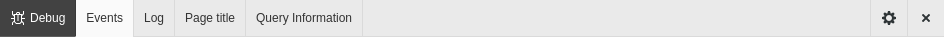
\includegraphics[width=0.85\linewidth]{ChangesForDevelopers/90265-ShowDispatchedEventsInAdminPanel.png}
	\end{figure}

\end{frame}

% ------------------------------------------------------------------------------
% Feature | 89738 | API for AJAX Requests

\begin{frame}[fragile]
	\frametitle{Änderungen für Entwickler}
	\framesubtitle{API für AJAX-Anforderungen}

	% decrease font size for code listing
	\lstset{basicstyle=\tiny\ttfamily}

	\begin{itemize}
		\item Die \textbf{Fetch-API} wurde eingeführt, um AJAX-Anfragen durchzuführen
			und TYPO3 weniger abhängig von jQuery zu machen.
		\item Die API bietet eine generische Definition von Request- und Response-Objekten
			(und anderen Dingen, die mit Netzwerkanforderungen zu tun haben).
		\item Dies wird von allen modernen Browsern unterstützt, siehe
			\href{https://developer.mozilla.org/en-US/docs/Web/API/Fetch_API}{Kompatibilitätstabelle}.
		\item Der TYPO3-Kern verwendet die neue API bereits im Install Tool, der FormEngine und
			den Kontextmenüs.
		\item Im
			\href{https://docs.typo3.org/c/typo3/cms-core/master/en-us/Changelog/10.3/Feature-89738-ApiForAjaxRequests.html}{Change Log}
			finden Sie einige Beispiele für die Verwendung der Fetch-API.

	\end{itemize}

\end{frame}

% ------------------------------------------------------------------------------
% Feature | 89650 | Allow line breaks in TCA descriptions

\begin{frame}[fragile]
	\frametitle{Änderungen für Entwickler}
	\framesubtitle{TCA-Beschreibungsfelder}

	\begin{itemize}
		\item Das Beschreibungsfeld im TCA kann nun Zeilenumbrüche enthalten, um lange Texte besser lesbar zu machen.
	\end{itemize}

\end{frame}

% ------------------------------------------------------------------------------
% Important | 90020 | Legacy BasicFileUtility and ExtendedFileUtility classes marked as internal

\begin{frame}[fragile]
	\frametitle{Änderungen für Entwickler}
	\framesubtitle{Klassen \texttt{BasicFileUtility} und \texttt{ExtendedFileUtility}}

	\begin{itemize}
		\item Die folgenden beiden Legacy-Klassen wurden als \textbf{internal} markiert
			und sollten nicht mehr verwendet werden:

			\begin{itemize}\small
				\item \texttt{TYPO3\textbackslash
					CMS\textbackslash
					Core\textbackslash
					Utility\textbackslash
					File\textbackslash
					BasicFileUtility}
				\item \texttt{TYPO3\textbackslash
					CMS\textbackslash
					Core\textbackslash
					Utility\textbackslash
					File\textbackslash
					ExtendedFileUtility}
			\end{itemize}

		\item Erweiterungsentwickler sollten stattdessen die Klassen \texttt{ResourceStorage}
			und \texttt{ResourceFactory} für die Verwaltung von Assets verwenden.

	\end{itemize}

\end{frame}

% ------------------------------------------------------------------------------
% Feature | 89139 | Add dependency injection support for console commands

\begin{frame}[fragile]
	\frametitle{Änderungen für Entwickler}
	\framesubtitle{Konsolenbefehle: Symfony DI Unterstützung}

	\begin{itemize}
		\item Befehlsabhängigkeiten können nun über den Konstruktor oder andere Injektionstechniken eingefügt werden.
		\item Fügen Sie das \texttt{console.command} Tag zu den Befehlsklassen hinzu.
		\item Verwenden Sie das Tag-Attribut \texttt{command}, um den Befehlsnamen anzugeben.
		\item Das optionale Tag-Attribut \texttt{schedulable} kann auf \texttt{false}
			gesetzt werden, um den Befehl aus dem TYPO3-Scheduler auszuschließen.

		\item Siehe
			\href{https://docs.typo3.org/c/typo3/cms-core/master/en-us/Changelog/10.3/Feature-89139-AddDependencyInjectionSupportForConsoleCommands.html}{change log}
			für ein Beispiel.
	\end{itemize}

\end{frame}

% ------------------------------------------------------------------------------
% Feature | 90168 | Introduce Modal Actions

\begin{frame}[fragile]
	\frametitle{Änderungen für Entwickler}
	\framesubtitle{Aktionsschaltflächen in Modalen}

	% decrease font size for code listing
	\lstset{basicstyle=\tiny\ttfamily}

	\begin{itemize}
		\item Modale Popups unterstützen jetzt Aktionsschaltflächen.
		\item Als Alternative zu der bestehenden \texttt{Trigger} -Option kann die neue Option
			\texttt{action} verwendet werden.
		\item Zum Beispiel:

\vspace{-0.4cm}
\begin{lstlisting}
Modal.confirm('Header', 'Some content', Severity.error, [
  {
    text: 'Based on trigger()',
    trigger: function () {
      console.log('Vintage!');
    }
  },
  {
    text: 'Based on action()',
    action: new DeferredAction(() => {
      return new AjaxRequest('/any/endpoint').post({});
    })
  }
]);
\end{lstlisting}

	\end{itemize}

\end{frame}

% ------------------------------------------------------------------------------
% Feature | 90471 | JavaScript Event API

\begin{frame}[fragile]
	\frametitle{Änderungen für Entwickler}
	\framesubtitle{JavaScript-Event-API}

	\begin{itemize}
		\item Eine neue Event-API ermöglicht JavaScript-Entwicklern eine stabile Schnittstelle zum Abhören von Ereignissen.
		\item Die API kümmert sich um häufige Fallstricke, wie z.B. die Delegierung von Veranstaltungen und saubere, unverbindliche Veranstaltungen.
		\item Jede \textit{Ereignisstrategie} bietet zwei Möglichkeiten, einen Zuhörer an ein Ereignis zu binden.
		\item Die Event-API bietet mehrere Strategien für den Umgang mit Event-Hörern.
		\item Siehe
			\href{https://docs.typo3.org/c/typo3/cms-core/master/en-us/Changelog/10.3/Feature-90471-JavaScriptEventAPI.html}{change log}
			für Beispiele und weitere Details.
	\end{itemize}

\end{frame}

% ------------------------------------------------------------------------------
